\documentclass{sig-alternate-10pt}

\usepackage{url, enumitem}

\begin{document}

\title{RaptorQ-based File Transfer Protocol}
\author{
  Yilong Li\\
  \texttt{yilongl@cs.stanford.edu}
  \and 
  Raejoon Jung\\
  \texttt{raejoon@stanford.edu}
  \and
  Yu Yan\\
  \texttt{yuyan0@stanford.edu}
}

\maketitle
\section{Introduction}

\section{Implementation}

\subsection{Reliable file transfer}

\subsection{Congestion control}

\section{Evaluation}
We test the tornado transfer implementation using emulated links generated by
Mahimahi \cite{mahimahi}. We measure the time spent for sending a file through
mahimahi with various link parameters. File transfer time via SCP is also
measured and compared. We observe the transfer time while changing three
parameters: (1) link loss, (2) link delay, and (3) file size. We fix the link
bandwidth to 12 Mbps. For each set of parameters, we ran 10 tests and report the
mean and the standard deviation in the following plots.

\subsection{Link loss test}

\begin{figure}[t]
  \centering
  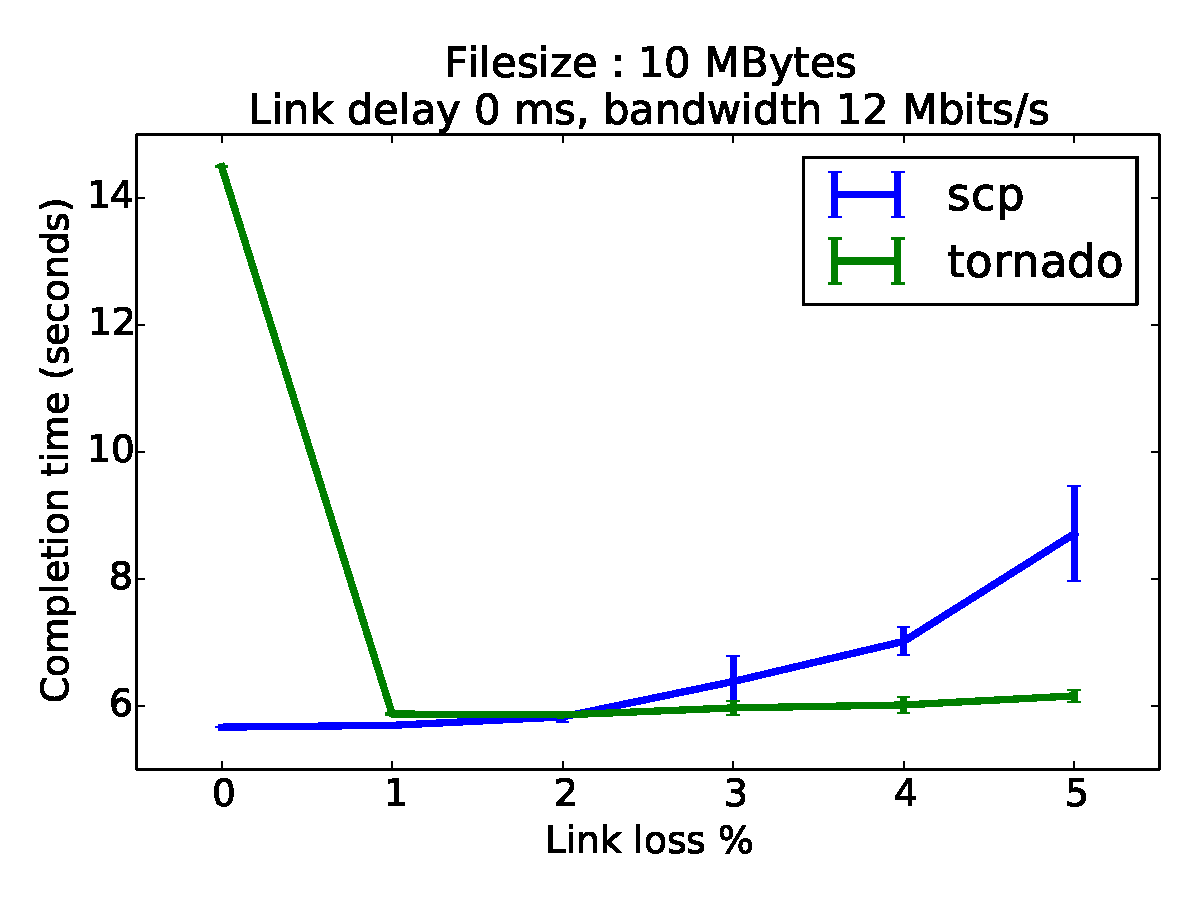
\includegraphics[width=0.5\textwidth]{loss-plot}
  \caption{Transfer time in lossy link}
  \label{f:loss-plot}
\end{figure}

Figure \ref{f:loss-plot} depicts the file transfer time using Tornado and SCP in
links with various packet loss probabilities. When the loss probability is
$\geq$ 1\%, transfer time of Tornado and SCP monotonically increase as the loss
probability increases. However the growth of Tornado's transfer time is much
less than SCP's transfter time. This results in a faster transfer time with
Tornado in loss proabilities of $\geq$ 2\% and the gap between the transfer time
of the two protocols gets wider as the loss proability increases.A

One interesting fact that we noticed is the transfer time using Tornado when
the loss probability is 0, i.e., the link is lossless. The average transfer time of
Torndao exceeds 14 seconds which is greater than $2\times$ compared to the case
when the link has 1\% loss probability. This is counter-intuitive since we
expect that packet loss can only deteriorate the operation of the file transfer
protocol. Currently, we do not have a clear explanation of this observation and
leave to future work to enhance the implementation to gracefully degrade
performance as the link probability increases.


\subsection{Link delay test}

\begin{figure}[t]
  \centering
  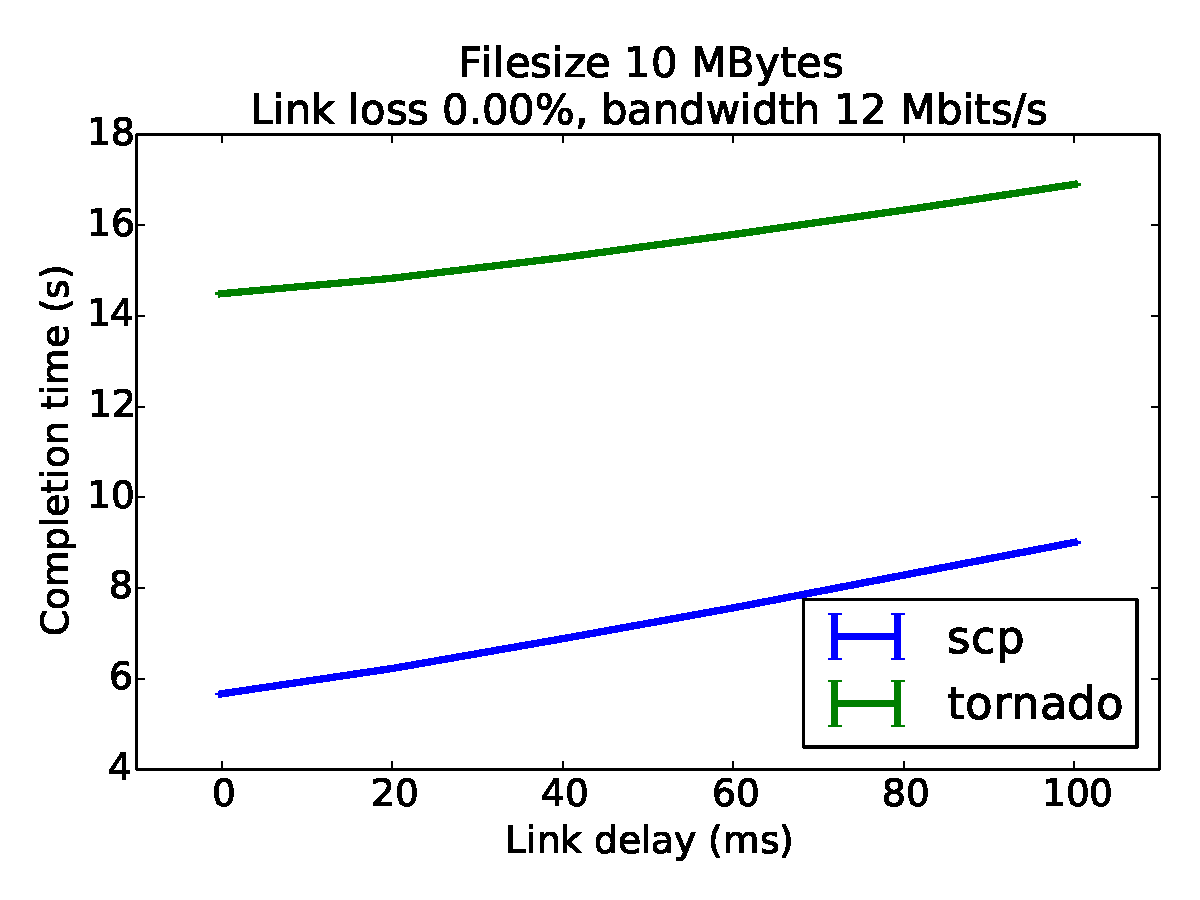
\includegraphics[width=0.5\textwidth]{delay-plot}
  \caption{Transfer time in link with delay. One way delays are stated.}
  \label{f:delay-plot}
\end{figure}

Figure \ref{f:delay-plot} shows the file transfer time in links with various
delay values. Throughout delay values from 0 to 100 ms, SCP maintains $\sim
2\times$ performance of Tornado. However, the difference of the transfer time is
almost constant in this delay range. In fact, the difference slightly decreases
as the delay increases. 

We first suspected the stage of computing intermediate symbols in Tornado to
cause this diffrence since this portion of the protocol requires extensive
computation and is done before the datagram transfer loop.  However, we have
confirmed that the progress of sending datagram was widely spread across the
application runtime rather than having a burst of datagram transfers after a
long pause as we expect if the intermediate symbol computation was the
bottleneck. From this observation, we expect this difference comes from the
inefficiency of our implmentation of the datagram transfer loop rather than
caused by the inefficiency of the design of the protocol.

\subsection{File size test}

\begin{figure}[t]
  \centering
  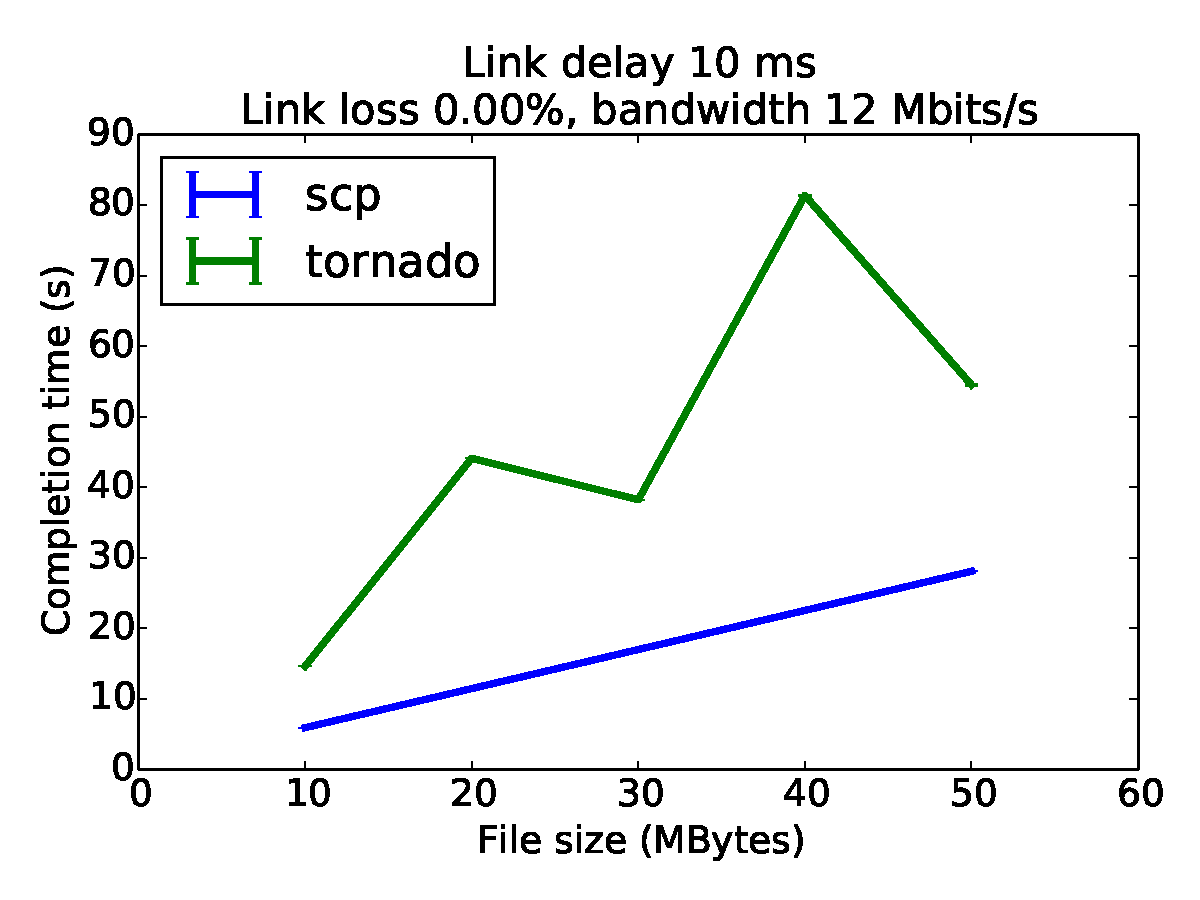
\includegraphics[width=0.5\textwidth]{filesize-plot}
  \caption{Transfer time with various file sizes}
  \label{f:filesize-plot}
\end{figure}

Figure \ref{f:filesize-plot} depcits the file transfer time using Tornado and
SCP with various file sizes when the link is lossless and has a one-way delay of
10ms. We tested with file sizes of 10, 20, 30, 40, and 50 MBs. In this range,
SCP transfers files faster than Tornado. Eventhough Tornado's transfer time does
not monotonically increase as the file size increases, the difference between
the transfer time of SCP and Tornado tends to increase.

The fact that Tornado's transfer time not increasing monotonically is also
noteworthy. We suspect that this is caused by the \texttt{libRaptorQ}'s internal
decision to set the number of blocks given a file size. Since we have no control
on the number of symbols per block since the size of a block can change
depending on \texttt{libRaptorQ}'s decision while we fix the symbol size. For
improvement, we can split the file into subfiles of fixed size and feed them
into multiple instances of encoders. Then we can expect regular performance
throughout the encoders. We leave the validation of the hypothesis and the
improvement for future work.

\section{Contribution}

\section{Reflection}

\section{Conclusion}

\cite{openrq}

\bibliography{finalreport}
\bibliographystyle{acm}

\end{document}
